\graphicspath{{chapters/04/images/}}
\chapter{Motif analysis}

\section{Introduction}

	\subsection{Definition}
	A DNA motif is a pattern of nucleotide sequences.
	They are usually associated to DNA-protein binding sites and to regulatory regions.
	They are a small pattern, usually between $5$ and $30bp$, that can recur many times in the genome and many times in the same gene.
	Motifs can be:

	\begin{multicols}{3}
		\begin{itemize}
			\item Standard.
			\item Palindromes.
			\item Gapped.
		\end{itemize}
	\end{multicols}

	\subsection{Functions}
	DNA motif functions include:

	\begin{multicols}{2}
		\begin{itemize}
			\item Sequence specific binding sites reached by transcription factors, nucleases and ribosomes.
			\item mRNA processing:

				\begin{itemize}
					\item Splicing: exonic splicing enhancer ESE.
					\item Editing: protospacer adjacent motif PAM, a DNA sequence that immediately follows the target DNA sequence of the Cas9 nuclease in the CRISPR system.
					\item Polyadenilation.
					\item Transcription termination.
				\end{itemize}

		\end{itemize}
	\end{multicols}

	\subsubsection{Degenerate motifs}
	Motifs in regulatory regions are often similar but variable: they are degenerate.
	Transcription factors are often pleiotropic, meaning that they regulate a lot of genes, but they need to be expressed at different levels.
	Degenerate motifs cause non-specific binding: a protein can bind genomic position different with respect to the one corresponding to the expected functional state.

\section{Motif search}
The objectives of motif search are to identify:

\begin{multicols}{3}
	\begin{itemize}
		\item Over-represented motifs in the genome.
		\item Motifs conserved in ortholog sequences.
		\item Sequences that can be candidates for transcription factor binding.
	\end{itemize}
\end{multicols}

Motifs can be represented as a consensus sequence or as profiles like positional matrices or hidden Markov models.

	\subsection{Consensus sequence}
	A consensus sequence represents the result of multiple sequence alignments with the goal of finding recurrent motifs across the sequences.
	This sequence can be potentially different from all input sequence: it presents only the most conserved sequences for each position.
	It is built such that it minimizes the distance from each input sequence at each position.
	It can be also written following a IUPAC notation.

	\subsection{Positional matrix}
	A positional matrix is an alternative way to represent a motif than the consensus sequences.
	The elements in the matrix represent all possible bases at each position.
	Example of these matrices are:

	\begin{multicols}{2}
		\begin{itemize}
			\item Position frequency matrix PFM or PSWM.
			\item Position probability matrix PPM or PFM.
			\item Position weight matrix PWM or PSSM.
		\end{itemize}
	\end{multicols}

	\begin{figure}[H]
		\centering
		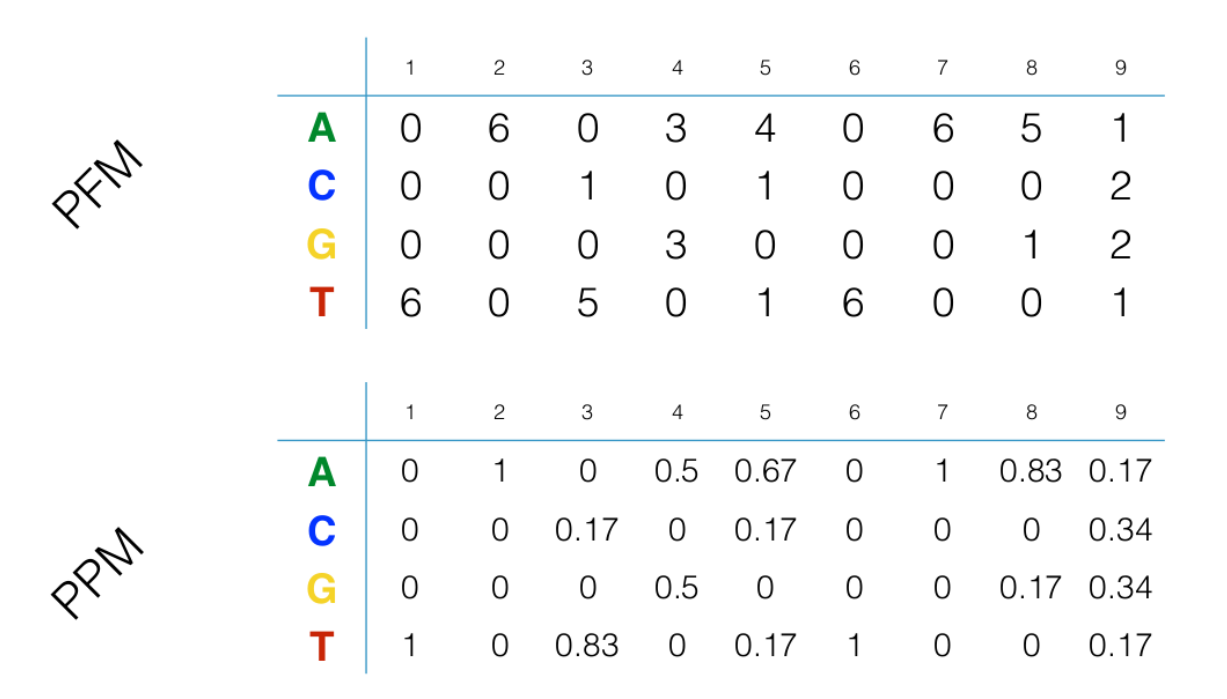
\includegraphics[scale=0.3]{matrices.png}
		\caption{Example of PFM and PPM}
		\label{fig:matrices}
	\end{figure}

		\subsubsection{Populating a position frequency matrix}
		In PFM, columns represent the position of the sequences and on the rows the nucleotide we expect to find on that position.
		So, when populating the matrix each column will contain the number of bases in the position that are counted.
		In this way the frequency at which a specific base at each specific position of multiple aligned sequences is counted.
		A position frequency matrix is computed as:

		$$M_{k,j} = \sum\limits_{i=1}^N\delta(X_{i,j} = k)$$

		Given:

		\begin{multicols}{2}
			\begin{itemize}
				\item $k$ the set of all symbols in the alphabet.
				\item $N$ the number of aligned sequences.
				\item $j$ iterates over the length of the sequence.
				\item $\delta$ is an indicator function, such that:

					$$\delta(X_{i,j} = k) = \begin{cases}1 &if X_{i,j} = k \\0 & otherwise\end{cases}$$

			\end{itemize}
		\end{multicols}

		\subsubsection{Populating a position probability matrix}
		A position probability matrix is very similar with respect to the position frequency matrix, with the exception that each cell represent the probability that in that sequence position a particular base will be found.
		PPM are useful because they are a normalization of the PFMs, making different matrices comparable with each other.
		Its cells are computed as:

		$$M_{k,j} = \frac{1}{N}\sum\limits_{i=1}^N\delta(X_{i,j} = k)$$

		Given:

		\begin{multicols}{2}
			\begin{itemize}
				\item $k$ the set of all symbols in the alphabet.
				\item $N$ the number of aligned sequences.
				\item $j$ iterates over the length of the sequence.
				\item $\delta$ is an indicator function, such that:

					$$\delta(X_{i,j} = k) = \begin{cases}1 &if X_{i,j} = k \\0 & otherwise\end{cases}$$

			\end{itemize}
		\end{multicols}

		\subsubsection{Assessing the probability that a sequence belong to a PPM}
		In PPMs, probabilities are calculated for each position independently.
		So, PPMs make the assumption that there is no statistical dependence between positions in the pattern.
		Dependence is not base specific but transcription factor specific.
		According to this PPMs can be considered models of a pattern that refers to a specific transcription factor.
		Meaning that searching if a function belongs to a PPM is equivalent to say how close the sequence is to that model.
		To assess the probability for a sequence $S$ to belong to a PPM the probabilities for each base $i$ found at each position $j$ are multiplied:

		$$P(S \in PPM) = \prod\limits_{j=1}^R M_{S_j, j}$$

		According to this equation if a sequence contains a base not read yet found, the probability would be zero.
		This would be incorrect, so the matrix needs to be corrected so that the probability of observing another base in a position is no longer zero.

		\subsubsection{Correcting PPMs}

			\paragraph{Laplace smoothing}
			Laplace smoothing introduces pseudocounts to allow to estimate probabilities in case of too few observations.
			A pseudocount is an integer or real amount added to the number of observed cases in order to change the expected probability.

			$$p_{i,\textit{empirical}} = \frac{x_i}{N} \qquad p_{i,\alpha\textit{-smoothed}} = \frac{x_i + \alpha}{N + \alpha d}$$

			Where $d$ is the number of observations added during Laplace smoothing.

			\paragraph{Adding a background model}
			Another way to correct PPMs is to add a background model.
			A background model reports the probabilities of observing a specific base at a specific position.
			Generally, in any position of the sequence each sequence has an expected probability of being observed of $25\%$.
			However, background models can vary, for example amino-acids instead of nucleotides or the GC content of the organism of the sequence can be exploited to build a more accurate model.
			With this a new matrix is computed as:

			$$M_{k,j} = \log_2\frac{M_{k,j}}{b_k}$$


			Where $b$ represent the background model.
			It is typically computed as:

			$$b_k = \frac{1}{|k|}$$

			And so is $0.25$ for nucleotides and $0.05$ for amino acids.

		\subsection{Assessing sequences' scores in a PWM matrix}
		To assess how close an input sequence is to the model implemented to a PWM a score should be computed.
		This is done by summing up the scores found in the columns for each base.
		The score indicates how much the sequence is different from a random sequence.
		This score is usually the measure used to search for positions where a putative binding for a transcription factor can be found.
		Indeed, for positions where the score, it might suggest that in that specific region a specific TF, embedded in the model, can bind to.
		Again, we assume we have pseudocounts embedded in our matrices to avoid zero scores.

		\begin{figure}[H]
			\centering
			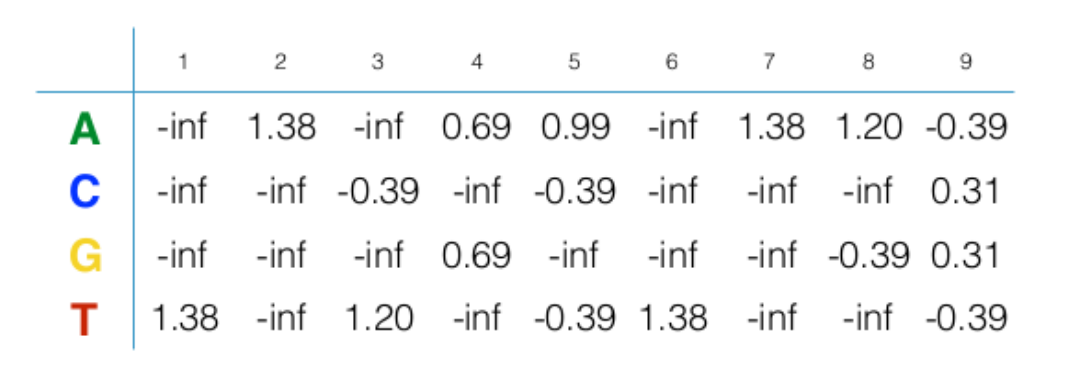
\includegraphics[scale=0.3]{pwm.png}
			\caption{Example of a PWM}
			\label{fig:pwm}
			\end{figure}


	\section{Hidden Markov model - HMM profile}
	Hidden Markov Models (HMM) are widely used in bioinformatics, as they provide for a useful tool when dealing with observational data.
	They are used for example to simulate signalling pathways.
	A Markov chain is a mathematical system that experiences transitions from one state to another according to certain probabilistic rules, and it represents the theoretical base for HMM.
	The possible future states are fixed and not based on how the process arrived at its present state.
	Meaning, the model has no memory of its past states and it does not matter how much time is spent one one state or the other.
	In a Markov chain, the state is directly visible to the observer: state transition probabilities are the only parameter.
	In a HMM instead, the state remains transparent, while the output, dependent on the state, is easily obtainable.

	To formalize these concepts: a HMM of the first order is defined as:
	\begin{multicols}{2}
		\begin{itemize}
			\item A finite set of states $S$.
			\item A discrete alphabet of symbols.
			\item A matrix of transition probabilities $T = P(i|j)$, the probability of transition from state $j$ to $i$
			\item A matrix of emission probabilities $T = P(X|i)$, the probability of $X$ emission in state $i$, the emission is what the user sees.
		\end{itemize}
	\end{multicols}

		\subsection{Assessing the probability that a sequence is generated by a HMM}
		The simplest way to build a model of a pattern representing a motif using HMM, is to build states that represent the different positions in the sequence and to associate some emission probabilities given each state.
		Given a set of sequences a set of transition, with each one representing a position in the sequence have to be modelled.
		In each state each nucleotide with probabilities proportional to the probabilities calculated in the position probability matrix are found.

		\begin{center}
			INSERIRE IMMAGINE
		\end{center}

		When assessing the probability that a sequence is generated by a HMM the probability of each state the sequence leads are summed up.
		This simple HMM can be extended with a background HMM.
		HMM for motif analysis become useful when dealing with indels or missing information, a very common scenario when performing multiple sequence alignment.
		Indels are modelled with edges connecting non-sequential states.
		The probability represented by the edge is proportional to the read count supporting the indel.

		\subsection{Match a sequence to a HMM profile}

		\begin{center}
			IMMAGINE
		\end{center}

		If the sequence $S$ is ATG, how many ways ways we can navigate this profile assuming match, insertion and deletion to match the seuence to the model?
		The simplest way is to assume all matches
		$$P(S|Model) = 0.8*0.1*0.7*0.2*0.6*0.1*0.9 = 0.0006048 \,\,\, \texttt{BMMME}$$
		But it is not the only possibility, for example:
		$$P(S|Model) = 0.8*0.1*0.2*0.4*0.25*0.75 = 0.0012 \,\,\, \texttt{BMDMIE}$$

				After generating the model, the probability that a sequence is generated by a HMM can be computed as:

		$$P(S|w) = \sum\limits_\pi P(S, \pi |w)$$

		Where:

		\begin{multicols}{3}
			\begin{itemize}
				\item $S$ is the sequence.
				\item $w$ are the probabilities parameters.
				\item $\pi$ are all possible paths.
			\end{itemize}
		\end{multicols}

		Finding the path with the highest probability means to find the best alignment to the HMM profile.
		Computing all paths in a brute-force way is clearly inefficient, but efficient algorithms to compute this probability like the Forward-Backward and the Viterbi exist.

		\begin{figure}[H]
			\centering
			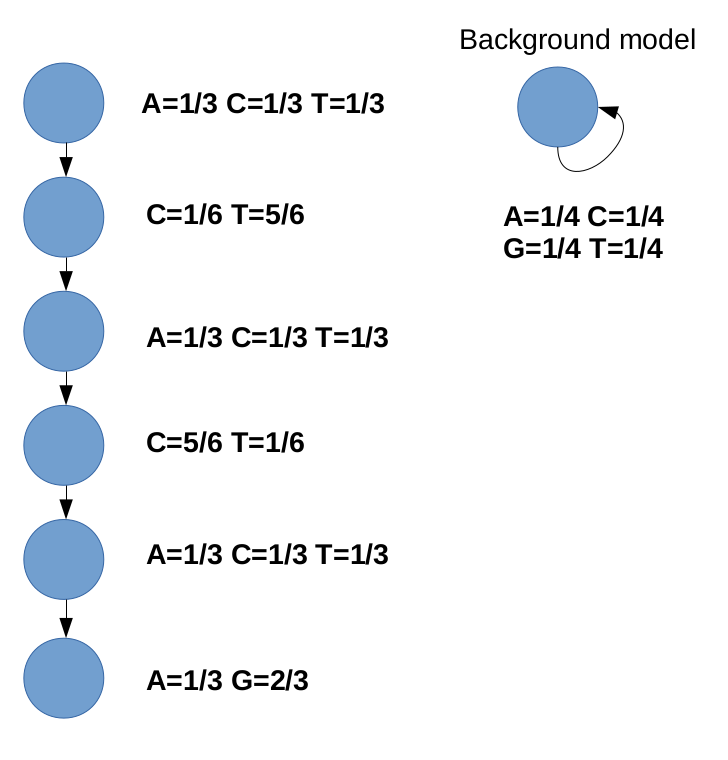
\includegraphics[scale=0.3]{HMM.png}
			\caption{Example of a HMM and background HMM models}
			\label{fig:HMM}
			\end{figure}

	\section{Sequence logos}
	Sequence logos are visual representation of positional matrices and simple HMM profiles.
	The height of each character in a sequence logo is proportional to its information content: $2$ bit if $1$ base occurs in all input sequences, $1$ if two bases occur and $0$ if all bases occur equally.
	The higher the variability, the lower the height of a specific base.
	In particular the height of base $b$ at position $l$ is computed as:

	$$f(b,l)R_{sequence}(l)$$

	Where:

	$$R_{sequence}(l) = 2-(H(l) + e(n))$$

	Such that $H(l)$ is the Shannon entropy and is computed as:

	$$H(l) = -\sum\limits_{b=a}^tf(b,l)\log_2 f(b,l)$$

	And

	$$e(n) = \frac{1}{\ln 2}\cdot \frac{4-1}{2n}$$

\section{Motif identification}
There are two types of motif identification: pattern matching and pattern discovery.

	\subsection{Finding known motifs - pattern matching}
	Pattern matching is the problem of finding known motifs, for example seeing if a binding of a protein $X$ to an upstream region of a gene $Y$ is significant.
	In order to find out whether a transcription factor matches a promoter the PFM matrix is used to compute a score for each sliding window.
	This scores can be plotted against a threshold, so as to identify regions able to support a putative binding.

		\subsubsection{Total binding affinity}
		Total binding affinity TBA is a cutoff-free method.
		The TBA is a method used to describe the affinity of a DNA sequence for a transcription factor described by a PFM with a single score.
		It takes into account binding sites of all possible affinities and considers the whole sequence, keeping into account both high and low affinity sites.
		For a sequence is computed as:

		$$a_{rw} = \sum\limits_{i=1}^{L-l+i}\max\bigg(\prod\limits_{j=1}^l \frac{P(w_j, r_{i+j-1})}{P(b, r_{i+j-1})}, \prod\limits_{j=1}^l\frac{P(w_{l-j+1}, r'_{i+j-1})}{P(b, r'_{i+j-1})}\bigg)$$

		Where:

		\begin{multicols}{2}
			\begin{itemize}
				\item $r$ is the sequence.
				\item $w$ is the $PFM$.
				\item $l$ is the length of $w$.
				\item $L$ is the length of $r$.
				\item $r_i$ is the nucleotide at position $i$.
				\item $r'_i$ is the nucleotide at position $i$ on the other strand.
				\item $P(w_j, r_i)$ is the probability to observe the given nucleotide $r_i$ at position $j$ of $w$.
				\item $P(b, r_i)$ is the background probability to observe the same nucleotide $r_i$.
			\end{itemize}
		\end{multicols}

	\subsection{Finding de novo motifs - pattern discovery}
	Pattern discovery is the problem of finding de novo motif, for example finding the motifs upstream of a specific gene $Y$ and which is the structure of these motifs.
	Given a set of sequences, the objective is to find the most represented motifs.
	Using the MEME suite it is possible to identify new sequences and through Jaspar (or other databses) they can be compared to already characterized transcription factors.
	Methods can be:

	\begin{multicols}{2}
		\begin{itemize}
			\item Exact: give optimal solution given specific parameters.
			\item Approximated: give suboptimal solution decreasing the computational burden.
				They are MULTIPROFILER, CONSENSUS, MEME, Gibbs sampler and MotifSampler for example.
		\end{itemize}
	\end{multicols}

		\subsubsection{Distance between a real motif and the consensus}
		The distance between a real motif and the consensus is generally less that that for two real motifs.
		The consensus sequence must be guessed and a scoring function to compare different guesses and choose the best one must be chosen.

		\subsubsection{Elements of the problem}
		The problem of finding de novo motifs can be formalized considering the following elements:

		\begin{multicols}{2}
			\begin{itemize}
				\item $n$ the length of each sequence.
				\item $DNA$, an array of size $t\times n$.
				\item $l$, the length of the motif or $l$-mer.
				\item $s_i$, the starting position of an $l$-mer in sequence $l$.
				\item $s = (s_1, s_2, \dots, s_t)$, an array of motifs starting position.
			\end{itemize}
		\end{multicols}

		If the starting positions $s$ are given, finding the consensus is easy.
		When those are not given, finding the best motif is solving the median string problem.

		\subsubsection{The median string problem}
		Given a set of $t$ DNA sequences the objective is to find a pattern that appears in all $t$ sequences with the minimum number of mutations.
		The Hamming distance is used, such that:

		$$d_h(v, w) = \#\ nucleotide\ pairs\ that\ do\ not match\ when\ v\ and\ w\ are\ aligned$$

		Then, for each DNA sequence $I$, all $d_h(v,x)$ are computed, where $x$ is an $l$-mer with starting position $s_i$.
		Then the minimum $d_h(v,x)$ among all $l$-mers of the sequence.
		The $TotalDistance(v,DNA)$ is the sum of the minimum Hamming distances for each DNA sequence $I$, so

		$$TotalDistance(v,DNA) = \min\limits_s d_h(v,s)$$

		Where $s$ is the set of starting positions.
